\lab{Algorithms}{SQL and Relational Databases}{SQL}
\objective{Understand concepts of a relational database and the fundamentals of the SQL language via SQLite.}
\label{lab:sql_rdb}

When working with large amounts of data, it is important to be able to quickly find and retrieve interesting information.
Fortunately, there is a way to handle such massive amounts of data in a reasonably efficient way.
A database allows us to store and retrieve data very quickly.
These databases are managed by a \emph{database management system}, or DBMS.
The DBMS is software that allows users to interact directly with the database.

\section*{Relational Databases}
A \emph{relational} database is paradigm for organizing data inside of a database.
This paradigm assumes that all data can be represented as a tuple of information.
A table, or \emph{relation}, is simply a set of tuples.
Each table has a \emph{schema} that defines the attributes of a tuple.
In the relational paradigm, there must be at least one column that can act as a primary key.
This can uniquely identify each tuple, or row, of the table.
It is common to use an ID number or other such unique information for the primary key.

\begin{figure}
\centering
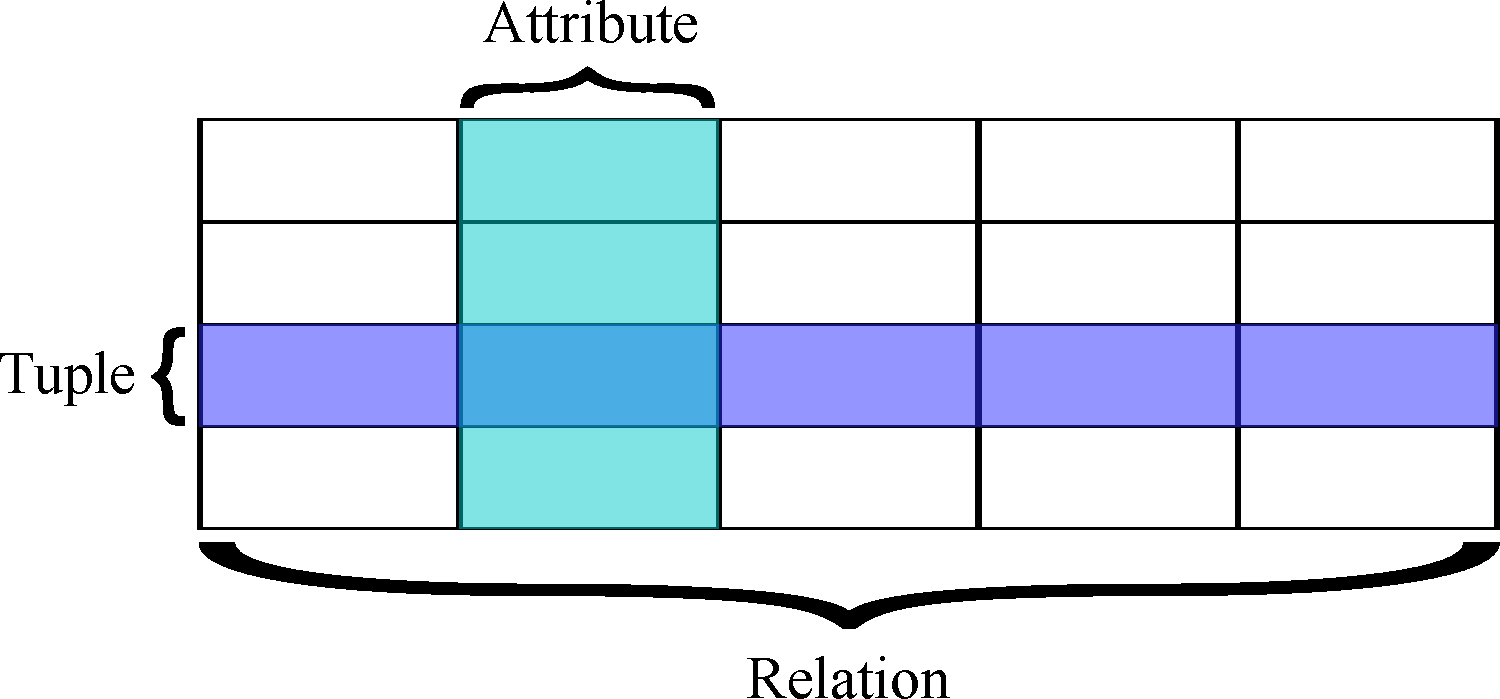
\includegraphics[width=\textwidth]{rdb_table.pdf}
\caption{Elements of a relation.}
\label{fig:relation}
\end{figure}

One important feature of databases are transactions.
Most relational databases are transactional databases.
The best way to conceptualize this is imagine that your database is like a bank.
Your connection the database is analogous to the bank teller.
When you make a deposit, or series of deposits, you are making a transaction.
This transaction should have certain properties.
These properties are succinctly captured in the acronym of ACID.
ACID compliance is an important feature transactional databases.
It describes the properties that a good database should have: atomic, consistent, isolation, and durable.
\begin{description}
\item[Atomic.] Each transaction should be all or nothing.  If some error occurs in the middle of a transaction, no changes are made to the database.  Changes are only made during error-free transactions.  This is especially useful if a transaction is interrupted due to power failure, or other type of unforeseen error.
\item[Consistent.] Ensure that the database is always left in a valid state.  This ensures that any transaction satisfies all rules and constraints of the database.
\item[Isolation.] The final effect of concurrent transactions it equivalent to the final effect of each transaction in serial.  This essentially means that if we run perform several transactions in parallel, none of the transactions can depend on each other.
\item[Durable.] Once a transaction is committed, the changes are permanent regardless of any errors that may happen later.
\end{description}

\section*{Introduction to SQL}
Most common DBMSs use a variant of the SQL language to interact with the database.
SQL is an acronym for \emph{Structured Query Language}.
While in general, SQL is not portable across databases, we will focus on the parts of SQL that are relatively common.
SQL consists of blocks of code called statements.
Each statement is made up of clauses which may or may not require predicates.
Predicates specify conditions that can limit the effect of a clause.
A SQL statement may either query (read-only), update (read-write), or insert (write only) information in the database.

Let's look at an example SQL statement
\begin{lstlisting}[language=SQL]
SELECT * FROM table WHERE id=3+1 AND name='Bob';
\end{lstlisting}
This statement includes a SELECT clause and a WHERE clause.
The WHERE clause contains two predicates: \texttt{id=3+1} and \texttt{name='Bob'}
These two predicates limit the effect of the SELECT clause because any resulting tuples in the table must satisfy both conditions.
This entire statement is classified as a query since it does not modify the database at all.



Databases are an essential part of computation.  We will learn how to use MySQL databases in this section.  MySQL is open-source software that is easy to use and free.  It also works well with Python.  All of this makes it a good choice for our applications.  Other options exist, but most of what we learn here will translate easily to other platforms.

We do not explain installation and setup of MySQL here.  See an appendix (TODO:  Make an appendix with a tutorial).

MySQL works by running a server that keeps track of databases and listens for queries.  There are several ways to interact with the server.  In this section, we will be using the MySQL terminal launched from the command line.  Let's begin by starting the server.  In your command prompt, navigate to the location of your MySQL installation. Now, type

Now that we are sure that the server is on, let's start the MySQL terminal so that we can talk to it.  From the command prompt, type


You should get a new prompt that looks like this

\begin{lstlisting}
Welcome to the MySQL monitor.  Commands end with ; or \g.
Your MySQL connection id is 1
Server version: 5.5.18 MySQL Community Server (GPL)

Copyright (c) 2000, 2011, Oracle and/or its affiliates. All rights reserved.

Oracle is a registered trademark of Oracle Corporation and/or its
affiliates. Other names may be trademarks of their respective
owners.

Type 'help;' or '\h' for help. Type '\c' to clear the current input statement.

mysql> 
\end{lstlisting}

You are now ready to start querying the server.

\section*{Basic Commands in MySQL}

\subsection{Creating Databases and Tables}

MySQL can store muliple databases, and each database will have several tables.  To see the databases in MySQL, we use the {\tt SHOW DATABASES;} command.

\begin{lstlisting}

mysql> SHOW DATABASES;
+--------------------+
| Database           |
+--------------------+
| information_schema |
| mysql              |
| performance_schema |
+--------------------+
3 rows in set (0.03 sec)

\end{lstlisting}

Note that the command ends with a semicolon. Every command we will see will also end with the same character.  Your terminal may show additional databases to these.  Each of these three databases store information about your installation of MySQL and the databases that are stored on the server.  They have their uses, but for now we will ignore them.

Now we will go over some basic queries that you can execute from the command line.  We want to be able to get data from MySQL server, but we don't have a database to get it from yet.  We can use the {\tt CREATE} command to create a new database.  In this example, we will create a student database with three tables.

\begin{lstlisting}
mysql>CREATE DATABASE students;
Query OK, 1 row affected (0.00 sec)

mysql> show databases;
+--------------------+
| Database           |
+--------------------+
| information_schema |
| mysql              |
| performance_schema |
| students           |
+--------------------+
4 rows in set (0.00 sec)

\end{lstlisting}

Now we add some tables to the students database.  First, we need to tell MySQL which database we want to work on with the {\tt USE} command.

\begin{lstlisting}

mysql> USE students;
Database changed

\end{lstlisting}

Now we use the {\tt CREATE} command to create a table and specify the column names of the table.

\begin{lstlisting}

mysql> CREATE TABLE student_information (StudentID INT NOT NULL, Name VARCHAR(20), SocSecurity INT, MajorCode INT);
Query OK, 0 rows affected (0.68 sec)

\end{lstlisting}

This creates a student information table with coloumns for each individuals student id, social security number, major, and name.  The arguments in parentheses are the column names followed by the datatype that entries in that column will take.  The {\tt INT} datatype allows up to 32-bit integers and {\tt VARCHAR(20)} allows strings of variable length up to 20 characters.  There are dozens of options to choose from.  The online MySQL documentation is a good resource to explore them.

Now we add another table that matches students to courses that they have taken and their grades.

\begin{lstlisting}

mysql> CREATE TABLE student_classes (StudentID INT NOT NULL, CourseID INT, Grade VARCHAR(2));
Query OK, 0 rows affected (0.26 sec)

\end{lstlisting}

\begin{problem}

In this problem you will create two new tables using the {\tt CREATE TABLE} syntax.  The first table will be called MajorInfo and have a columns called MajorCode and MajorName.  MajorCode should have the INT datatype and MajorName should be VARCHAR(20).

The second table will be called CourseInfo and have columns called CourseID and CourseName, also INT and VARCHAR(20) respectively.

\end{problem}

\subsection{Inserting Data}

In this section we will insert data into the tables that we have created.  First we will show how to manually add data using the {\tt INSERT} command.  {\tt INSERT} requires that we specify which table that we wish to modify and the values for each column.  For example

\begin{lstlisting}
mysql> INSERT INTO student_information VALUES(55, "John Smith", 372897382, 2);
Query OK, 1 row affected (0.20 sec)
\end{lstlisting}

We may also remove the line we just inserted using the {\tt DELETE} command.

\begin{lstlisting}

mysql> DELETE FROM student_information WHERE StudentID=55;
Query OK, 1 row affected (0.16 sec)

\end{lstlisting}

These commands are useful for table maintenance or where it may be automated, but MySQL is a very powerful tool for dealing with large amounts of data.  Manually inserting and deleting in such a table is ornerous in even simple cases and essentially impossible for a moderately sized table.  If we have some data in a file on our computer, we may use the {\tt LOAD} command to automatically move it into our database.

\begin{lstlisting}

mysql> LOAD DATA LOCAL INFILE "./students.dat" INTO TABLE student_information FIELDS TERMINATED BY ",";
Query OK, 10 rows affected (0.07 sec)

\end{lstlisting}

{\tt LOCAL INFILE} specifies that we are a loading file from a location on our local machine.  We then specify the path to the file and which table to load the data into.  Finally, we specify what character separates the columns.  Even for large files this operation moves very fast.

\begin{problem}

Download students.dat, class\_info.dat, classes.dat, and major\_info.dat and use the {\tt LOAD} command to insert the data in each into student\_information, ClassInfo, student\_classes and MajorInfo respectively.

\end{problem}

\begin{problem}

Using python, write a program that will accepts a number of rows and returns a 10 column matrix with the specified number of rows and write it to a file with each column separated by commas.  The first column should be in ascending numeric order, but the others should have random numbers in them.  Generate matrices with 100, 1000, 10000, and 100000 rows.  Load each into a different table in a new database and time the load operation.  How does the time increase?

\end{problem}

\section{Querying and Joining Tables}

Now that we have loaded data in the form of our student database we will learn to query and join the tables.  The first command that we will use is {\tt SELECT}, which returns specified rows of a table.  For example

\begin{lstlisting}
mysql> SELECT Name FROM student_information;
+---------------------+
| Name                |
+---------------------+
|  Jared Webb         |
|  Alexander Zaitzeff |
|  Rachel Suggs       |
|  Jeff Humphreys     |
|  Abe Frandsen       |
|  Tyler Jarvis       |
|  Jessica Purcell    |
|  Janice Joplin      |
|  John Lennon        |
|  Tupac Shakur       |
+---------------------+
10 rows in set (0.00 sec)
\end{lstlisting}

After {\tt SELECT} we specify a column and a table to query, and MySQL returns the requested rows.  We may also add conditions to our command to get more refined results.

\begin{lstlisting}

mysql> SELECT Name FROM student_information WHERE StudentID = 4;
+-----------------+
| Name            |
+-----------------+
|  Jeff Humphreys |
+-----------------+
1 row in set (0.00 sec)

\end{lstlisting}

Or we may select more than one column

\begin{lstlisting}

mysql> SELECT Name, SocSecurity FROM student_information WHERE StudentID = 4;
+-----------------+-------------+
| Name            | SocSecurity |
+-----------------+-------------+
|  Jeff Humphreys |   736452198 |
+-----------------+-------------+
1 row in set (0.00 sec)

mysql> SELECT * FROM student_information WHERE StudentID = 4;
+-----------+-----------------+-------------+-----------+
| StudentID | Name            | SocSecurity | MajorCode |
+-----------+-----------------+-------------+-----------+
|         4 |  Jeff Humphreys |   736452198 |         3 |
+-----------+-----------------+-------------+-----------+
1 row in set (0.00 sec)

mysql> SELECT * FROM student_information;
+-----------+---------------------+-------------+-----------+
| StudentID | Name                | SocSecurity | MajorCode |
+-----------+---------------------+-------------+-----------+
|         1 |  Jared Webb         |   123456789 |         1 |
|         2 |  Alexander Zaitzeff |   987654321 |         1 |
|         3 |  Rachel Suggs       |   431256789 |         2 |
|         4 |  Jeff Humphreys     |   736452198 |         3 |
|         5 |  Abe Frandsen       |   172645382 |         4 |
|         6 |  Tyler Jarvis       |   174382645 |         3 |
|         7 |  Jessica Purcell    |   827635142 |         2 |
|         8 |  Janice Joplic      |   987263512 |         1 |
|         9 |  John Lennon        |   192837641 |         3 |
|        10 |  Tupac Shakur       |   192837412 |         2 |
+-----------+---------------------+-------------+-----------+
10 rows in set (0.00 sec)

\end{lstlisting}

We may join tables by columns using the {\tt INNER JOIN} command.  This is a very powerful tool for uniting data across many tables.  In MySQL we can use {\tt INNER JOIN} in conjunction with {\tt SELECT} to query data across many tables into place.  For example we can inner join student\_classes and student\_information on the StudentID column to display student information and grades in one table.

\begin{lstlisting}

mysql> SELECT * FROM student_information INNER JOIN student_classes ON student_information.StudentID = student_classes.StudentID;
+-----------+---------------------+-------------+-----------+-----------+---------+-------+
| StudentID | Name                | SocSecurity | MajorCode | StudentID | ClassID | Grade |
+-----------+---------------------+-------------+-----------+-----------+---------+-------+
|         1 |  Jared Webb         |   123456789 |         1 |         1 |       4 |  C    |
|         1 |  Jared Webb         |   123456789 |         1 |         1 |       3 |  B    |
|         2 |  Alexander Zaitzeff |   987654321 |         1 |         2 |       4 |  A    |
|         2 |  Alexander Zaitzeff |   987654321 |         1 |         2 |       3 |  A    |
|         3 |  Rachel Suggs       |   431256789 |         2 |         3 |       2 |  C    |
|         2 |  Alexander Zaitzeff |   987654321 |         1 |         2 |       1 |  B    |
|         4 |  Jeff Humphreys     |   736452198 |         3 |         4 |       1 |  A    |
|         5 |  Abe Frandsen       |   172645382 |         4 |         5 |       2 |  C    |
|         5 |  Abe Frandsen       |   172645382 |         4 |         5 |       3 |  C    |
|         6 |  Tyler Jarvis       |   174382645 |         3 |         6 |       4 |  D    |
|         6 |  Tyler Jarvis       |   174382645 |         3 |         6 |       2 |  A    |
|         6 |  Tyler Jarvis       |   174382645 |         3 |         6 |       1 |  B    |
|         7 |  Jessica Purcell    |   827635142 |         2 |         7 |       2 |  A    |
|         7 |  Jessica Purcell    |   827635142 |         2 |         7 |       1 |  C    |
|         8 |  Janice Joplic      |   987263512 |         1 |         8 |       2 |  D    |
|         8 |  Janice Joplic      |   987263512 |         1 |         8 |       1 |  A    |
|         5 |  Abe Frandsen       |   172645382 |         4 |         5 |       4 |  A    |
|         9 |  John Lennon        |   192837641 |         3 |         9 |       2 |  B    |
|         9 |  John Lennon        |   192837641 |         3 |         9 |       3 |  C    |
|        10 |  Tupac Shakur       |   192837412 |         2 |        10 |       1 |  A    |
|        10 |  Tupac Shakur       |   192837412 |         2 |        10 |       2 |  A    |
+-----------+---------------------+-------------+-----------+-----------+---------+-------+
21 rows in set (0.05 sec)

\end{lstlisting}

By specify columns, we can display the grades of one student.

\begin{lstlisting}

mysql> SELECT Name, Grade FROM student_information INNER JOIN student_classes ON student_information.StudentID = student_classes.StudentID WHERE student_information.StudentID=6;
+---------------+-------+
| Name          | Grade |
+---------------+-------+
|  Tyler Jarvis |  D    |
|  Tyler Jarvis |  A    |
|  Tyler Jarvis |  B    |
+---------------+-------+
3 rows in set (0.05 sec)

\end{lstlisting}

\begin{problem}

Use {\tt INNER JOIN} and {\tt SELECT} to display the student\_information table, but show the students majors and classes instead of ClassID and MajorID.

\end{problem}

